\begin{figure}
	\begin{minipage}{0.49\linewidth}
		\center
		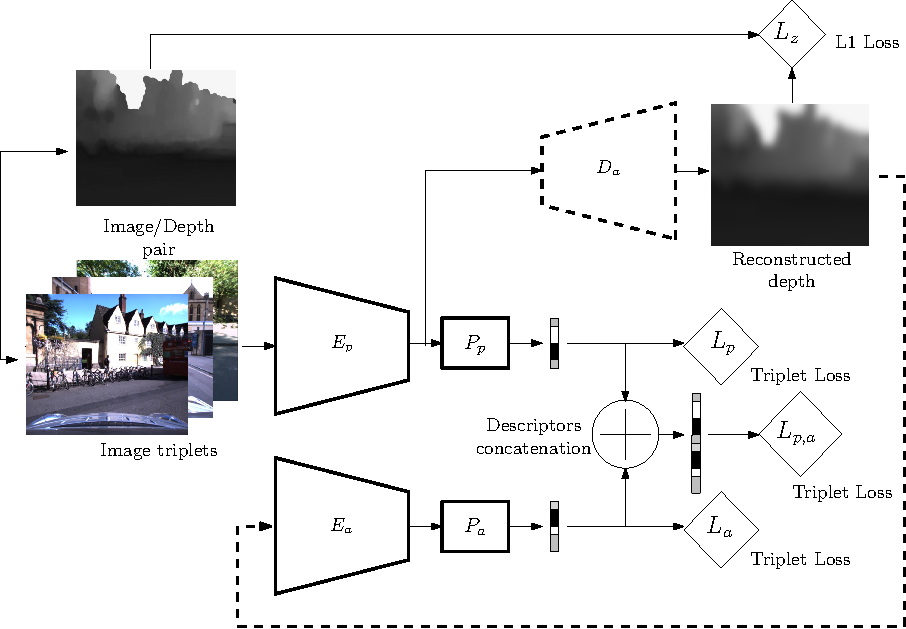
\includegraphics[width=\linewidth]{method/our_method_training}
		\caption[Image descriptors training with auxiliary depth data]{\label{fig:our_method} \textbf{Image descriptors training with auxiliary depth data (our work):} two encoders are used for extracting deep features map from the main image modality and the auxiliary reconstructed depth map (inferred from our deep decoder). These features are used to create intermediate descriptors that are finally concatenated in one final image descriptor.}	
	\end{minipage}\hfill
	\begin{minipage}{0.49\linewidth}
		\center
		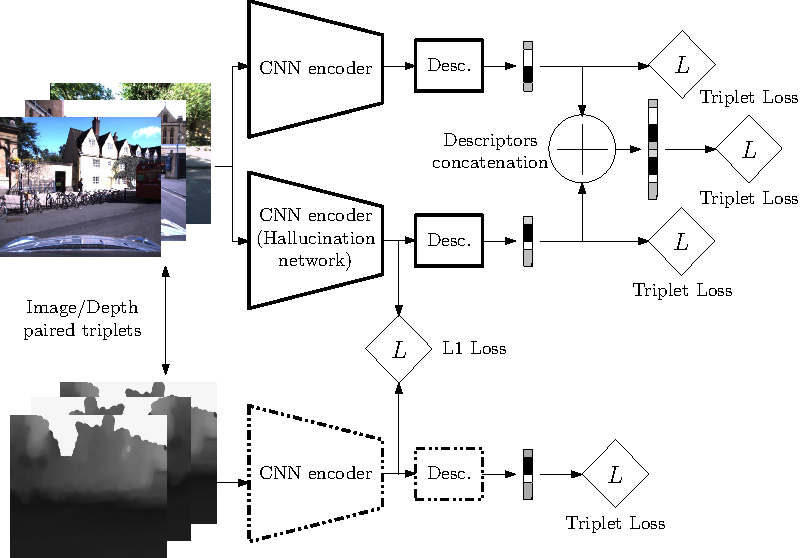
\includegraphics[width=\linewidth]{method/hall_method_training}
		\caption[Hallucination network for image descriptors learning]{\label{fig:hall_method} \textbf{Hallucination network for image descriptors learning:} we train an hallucination network, inspired from~\cite{Hoffman2016}, for the task of global image description. Unlike the proposed method (see figure~\ref{fig:our_method}), hallucination network reproduces feature maps that would have been obtained by a network trained with depth map rather than the deep map itself.}
	\end{minipage}
	
\end{figure}
	